\documentclass[english]{article}
\usepackage[utf8]{inputenc}
\usepackage[T1]{fontenc}
\usepackage{afterpage}
\usepackage{graphicx}
\usepackage{tabularx}
\usepackage{geometry}
\usepackage{listings}
\usepackage{amsmath}
\usepackage{xcolor}
\usepackage{babel}
\usepackage{float}
\usepackage{multirow}
\usepackage{array}
\newcolumntype{C}{>{\centering\arraybackslash}m{2cm}}
% Add in specific class to use \subsubsubsection, \paragraph, \subparagraph
\usepackage{titlesec}
\titleclass{\subsubsubsection}{straight}[\subsection]
\newcounter{subsubsubsection}[subsubsection]
\renewcommand\thesubsubsubsection{\thesubsubsection.\arabic{subsubsubsection}}
\renewcommand\theparagraph{\thesubsubsubsection.\arabic{paragraph}} % optional; useful if paragraphs are to be numbered
\titleformat{\subsubsubsection}
  {\normalfont\normalsize\bfseries}{\thesubsubsubsection}{1em}{}
\titlespacing*{\subsubsubsection}
{0pt}{3.25ex plus 1ex minus .2ex}{1.5ex plus .2ex}
\makeatletter
\renewcommand\paragraph{\@startsection{paragraph}{5}{\z@}%
  {3.25ex \@plus1ex \@minus.2ex}%
  {-1em}%
  {\normalfont\normalsize\bfseries}}
\renewcommand\subparagraph{\@startsection{subparagraph}{6}{\parindent}%
  {3.25ex \@plus1ex \@minus .2ex}%
  {-1em}%
  {\normalfont\normalsize\bfseries}}
\def\toclevel@subsubsubsection{4}
\def\toclevel@paragraph{5}
\def\toclevel@paragraph{6}
\def\l@subsubsubsection{\@dottedtocline{4}{7em}{4em}}
\def\l@paragraph{\@dottedtocline{5}{10em}{5em}}
\def\l@subparagraph{\@dottedtocline{6}{14em}{6em}}
\makeatother
\setcounter{secnumdepth}{4}
\setcounter{tocdepth}{3}
\geometry{left=1.5in, right=1.5in, top=1in, bottom=1.25in}
\titleformat{\section}{\clearpage\normalfont\Large\bfseries}{\thesection}{1em}{}
\usepackage{hyperref}
\hypersetup{
    colorlinks=true,
    linkcolor=black,
    filecolor=magenta,      
    urlcolor=blue,
    pdfpagemode=FullScreen,
}

\lstdefinestyle{mystyle}{
    language=Python, % Specify the programming language
    basicstyle=\ttfamily, % Set the font style (typewriter font)
    keywordstyle=\color{blue}, % Define keywords color
    commentstyle=\color{green}, % Define comments color
    numbers=none, % Display line numbers
    numberstyle=\tiny\color{gray}, % Line number font style
    breaklines=true, % Enable line wrapping
    frame=single, % Add a frame around the code
    tabsize=4 % Set the tab size
}

\definecolor{gray}{rgb}{0.5,0.5,0.5}

\begin{document}

\begin{titlepage}
\centering

\vspace{4cm} 

\Huge

Üzleti Intelligencia

\vspace{2cm} 

\Large

Megerősítéses tanulás - beadandó feladatok

\vspace{0.5cm}

2023 % Dátum

\vspace{2cm} 

\normalsize

A feladatok 1-3 skálán vannak osztályozva nehézség szerint, ahol 1 a legkönnyebb és 3 a legnehezebb. A beadás feltételei megegyeznek az előző beadandó feladatéval. Késő beadás nem lehetséges, a dátum beadásakor feltöltött anyagok fognak leosztályozásra kerülni. Minden további információ a tantárgyi útmutatóban és az órán elhangzottakban találhatóak.
\par\medskip
A feladatok hozzárendelése úgy történik, hogy a két beadandó feladatból összesen 4 nehézség pontot kelljen teljesítenie minden hallgatónak. Tehát aki az első beadandóban 1-es nehézségű feladatot kapott, ebben a körben 3-as nehézségűt kell kapnia.
\par\medskip
\textbf{Az elégséges jegy feltétele, hogy a program hiba nélkül lefusson. Hibaüzenettel beadva a program nem éri el az elvárt színvonalat.}
\end{titlepage}

\section{Osztályozás (1)}
\begin{center}
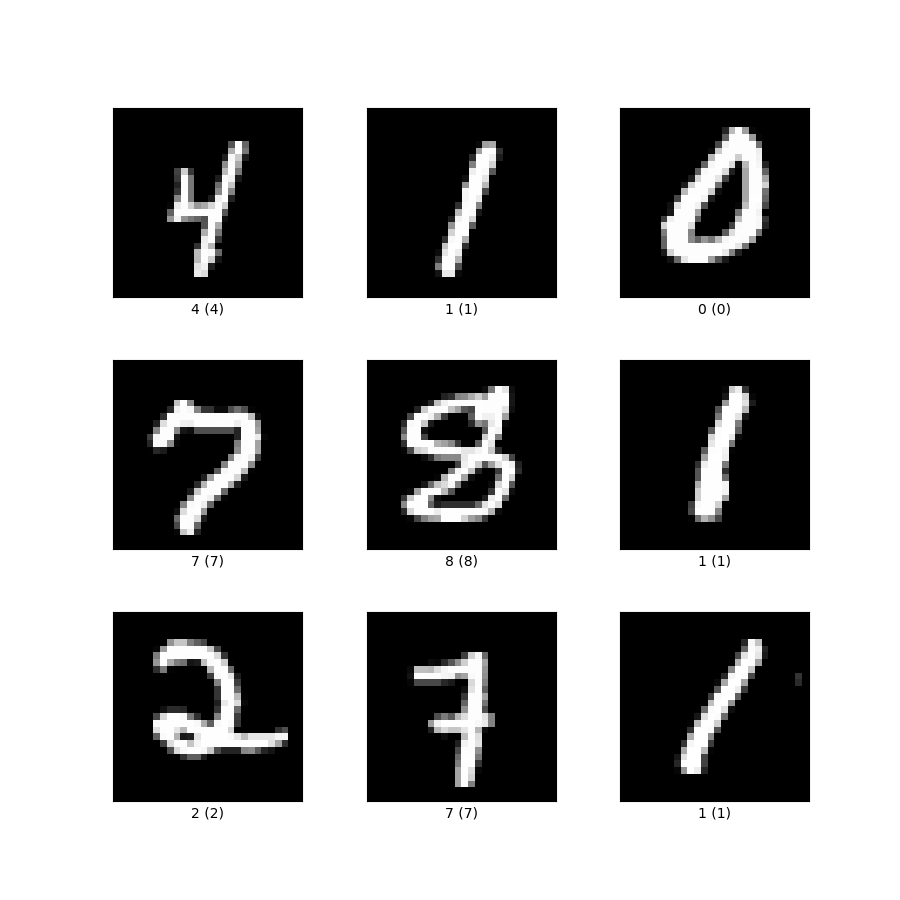
\includegraphics[width=5cm, keepaspectratio]{images/mnist.png}
\end{center}
\begin{enumerate}
	\item Töltse be az MNIST adathalmaz teszt képeit.
	\item Töltsön be egy tetszőleges képfeldolgozó modellt (ajánlat: pytorch resnet50 előre tanított modell).
	\item Használja fel a modellt arra, hogy predikciót végezzen az MNIST képeken.
	\item Adja meg az osztályozás \emph{precision}, \emph{recall} mutatóit. 
	\item Adja meg, melyik a két leginkább összekevert számjegy egy normalizált korrelációs mátrix alapján.
	\item Ábrázoljon ezek közül néhány helyesen osztályozottat, hamis pozitívat és hamis negatívat. 
	\item Írja le az eljárás elméleti alapjait és saját tapasztalatait egy Jupyter markdown cellában.
\end{enumerate}

\section{Objektum detekció (1)}
\begin{center}
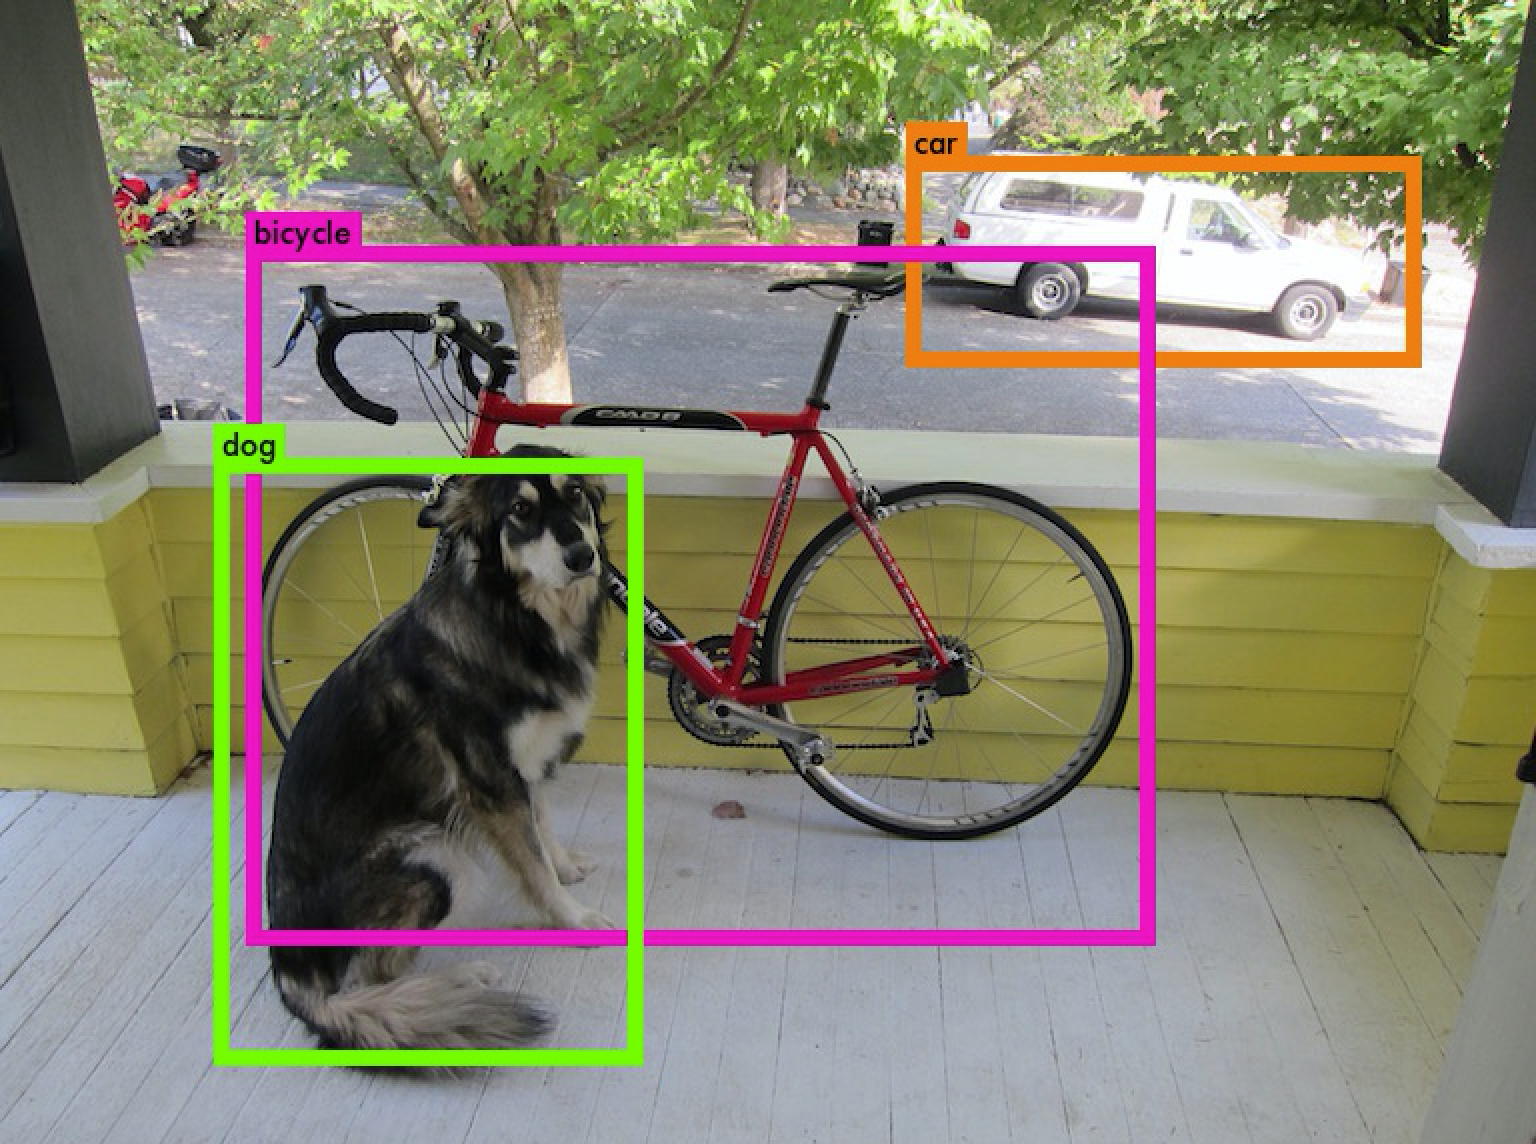
\includegraphics[width=5cm, keepaspectratio]{images/object_detection.png}
\end{center}
\begin{enumerate}
	\item Töltse be a PASCAL VOC adathalmaz 100 véletlenszerűen kiválasztott képét és a hozzájuk tartozó objektum kereteződoboz címkéket. A véletlen mintavételhez használjon tetszőleges bázisértéket (seed).
	\item Végezzen a képeken objektum detekciót egy tetszőleges objektum detektor modellel (Faster R-CNN, Detectron2).
	\item Mérje meg a megfelelő módszerrel és adja meg az osztályozás átlagos IoU értékét az összes osztályra. 
	\item Mérje meg a megfelelő módszerrel és adja meg az osztályozás átlagos IoU értékét az egyes osztályra külön-külön.
	\item Ábrázoljon diagramon néhány predikción.
	\item Írja le az eljárás elméleti alapjait és saját tapasztalatait egy Jupyter markdown cellában.
\end{enumerate}

\section{Egyed szegmentáció (2)}
\begin{center}
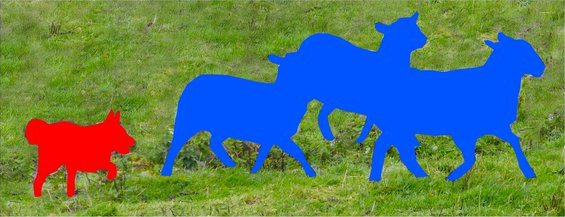
\includegraphics[width=8cm, keepaspectratio]{images/semantic_segmentation.jpg}
\end{center}
\begin{enumerate}
	\item Töltse le a lokális tárhelyre a PASCAL VOC adathalmazt és a hozzá tartozó annotációkat.
	\item Válasszon ki 100 képet véletlenszerűen. A véletlenszerű mintavételhez válasszon tetszőleges bázisértéket (seed).
	\item Töltsön be egy tetszőleges modellt, amelyik képes egyed szegmentációt végezni és a tanult osztályai megfelelnek az adathalmaz osztályainak. 
	\item Végezzen egyed szegmentációt a képeken. 
	\item Hasonlítsa össze a valós és becsült szegmentációs maszkokat. Adja meg mekkora osztályonként az átlagos IoU érték. 
	\item Ábrázoljon diagramon néhány predikciót/valós érték összehasonlítást.
	\item Írja le az eljárás elméleti alapjait és saját tapasztalatait egy Jupyter markdown cellában.
\end{enumerate}

\section{Arcfelismerés (2)}
\begin{center}
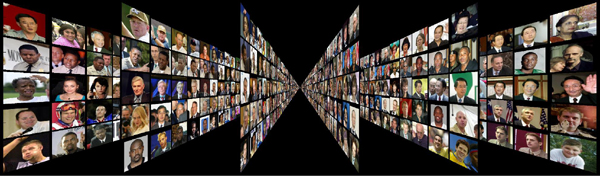
\includegraphics[width=8cm, keepaspectratio]{images/lfw.jpg}
\end{center}
\begin{enumerate}
	\item Töltse be az \href{http://vis-www.cs.umass.edu/lfw/#download}{LFW} (Labeled Faces in the Wild) adathalmaz 200 véletlenszerűen kiválasztott képét úgy, hogy személyenként legalább 5 képet tartalmazzon. Mentse el, hogy melyik kép kihez tartozik. Használjon egy tetszőleges bázisértéket (seed) a választáshoz.
	\item Végezzen arcfelismerést az mintázott adathalmazon. Mentse el az egyes arcok beágyazóvektorait a nevekhez tartozóan. 
	\item Szeparálja az adathalmazt 150-50 arányban tanító és teszt adatokra úgy, hogy minden személyből kerüljön mindkét adathalmazba.
	\item Mérje le a pontosságot a teszt adathalmazon: adja meg, melyik beágyazóvektorhoz melyik a leginkább hasonló (ehhez szükség lesz egy vektor-vektor távolság függvényre pl. koszinusz hasonlóság). Ebben az esetben fel lehet használni egy tetszőleges gépi tanulás modellt is, ami képes megtanulni ilyen jellemzőket. 
	\item Adja meg az arcfelismerés pontosságát (mekkora arányban sikerült a vektorokhoz tartozó neveket összepárosítani).
	\item Írja le az eljárás elméleti alapjait és saját tapasztalatait egy Jupyter markdown cellában.
\end{enumerate}

\section{Pózfelismerés (2)}
\begin{center}
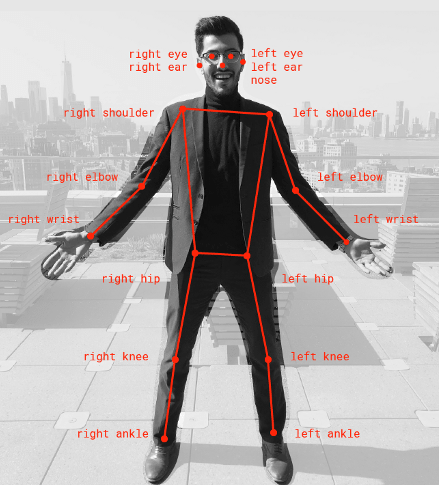
\includegraphics[width=7cm, keepaspectratio]{images/pose_detection.png}
\end{center}
\begin{enumerate}
	\item Töltsön le egy tetszőleges videót. Nem kell hosszúnak és nagy felbontásúnak lennie, viszont szükséges embereknek szerepelnie rajta. 
	\item Töltsön be egy tetszőleges gépi tanulás modellt előretanított súlyokkal, ami képes emberi pózfelismerést végezni.
	\item Olvassa a videót OpenCV segítségével és végezzen minden képkockán emberi pózfelismerést.
	\item Írja ki az eredményt egy új videóba. 
	\item Írja le az eljárás elméleti alapjait és saját tapasztalatait egy Jupyter markdown cellában.
\end{enumerate}

\end{document}
















